\begin{frame}
    \frametitle{S-CTM - Example}
    \metroset{block=fill}
    \begin{block}{Diverge network}
    \begin{columns}[c]
    \begin{column}{0.4\textwidth}
      \begin{figure}
      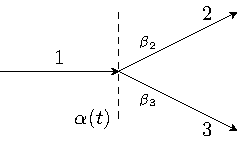
\includegraphics[scale=0.6]{fig_51_diverge3}
      \end{figure}
    \end{column}
    \begin{column}{0.4\textwidth}
      $
      \onslide<1->{\dot{\rho}_1 = }
      \dfrac{
      \onslide<2->{f_1^{in} - f_1^{out} }
      \onslide<3->{{\color{blue}u_1(t)} }
      }{L_1}
      $
    \end{column}
    \end{columns}
    \end{block}
    \begin{block}<4->{4--roads intersection}
    \begin{columns}[c]
    \begin{column}{0.3\textwidth}
        \hbox{\hspace{3em}
        \begin{tikzpicture}[>=stealth,scale=0.6]
        \draw[->] (0,0)--(2,0) node[midway, above, color=black]  {\scriptsize$1$};
        \draw[->] (2,2)--(2,0) node[midway, left, color=black] {\scriptsize$2$};
        \draw[->] (2,0)--(4,0) node[near end, above, color=black] {\scriptsize$3$} node[midway, below, color=black] {\scriptsize $\beta_3$};
        \draw[->] (2,0)--(2,-2) node[near end, right, color=black] {\scriptsize$4$} node[near start, right, color=black] {\scriptsize $\beta_4$};
        \coordinate (a) at (1,-1);
        \coordinate (b) at (3.3,1);
        \draw[dashed] (3,1)--(1,-1) node[above left = -5pt  of a] {\scriptsize$u$(t)};% node[above left = -5pt of b] {$\alpha^{(2)}$};
        \end{tikzpicture}}
    \end{column}
    \begin{column}{0.7\textwidth}
      $
      \dot{\rho}_3 = \frac{1}{L_3} \Big(f_3^{in} - f_3^{out}\Big)  = \frac{ \Big(\big( \onslide<6->{{\color{blue}u_1(t)}} \onslide<5->{{\color{black}f_1^{out}}\beta_{13}} + \onslide<6->{{\color{blue}\big(1-u_1(t)\big)}} \onslide<5->{{\color{black}f_2^{out}\beta_{23}}} \big) - f_3^{out}  \Big)}{L_3}
      $
    \end{column}
    \end{columns}
    \end{block}
\end{frame}